\documentclass[sigconf,nonacm]{acmart}

%% Remove ACM copyright block completely
\settopmatter{printacmref=false}
\setcopyright{none}
\renewcommand\footnotetextcopyrightpermission[1]{}
\pagestyle{plain}

%% Packages
\usepackage{tikz}
\usepackage{pgfplots}
\pgfplotsset{compat=1.18}
\usetikzlibrary{arrows.meta,positioning,shapes.geometric}
\usepackage{booktabs}
\usepackage{amsmath}
\usepackage{enumitem}
\usepackage{microtype}

\begin{document}

\title{Explainable Music Genre Classification via\\Multi-Concept Bottleneck Representations}
\subtitle{CS3631 Project Proposal}

\author{%
Anupama Wickramaratne$^{\ddagger}$,
Thevindu Fernando$^{\ddagger}$,
Tharupahan Jayawardana$^{\ddagger}$,
Dehan Wijesinghe$^{\ddagger}$,
Senindu Dinapura$^{\ddagger}$}
\affiliation{%
  \institution{Dept.\ of Computer Science \& Engineering, University of Moratuwa, Sri Lanka}
  \country{}
}
\email{\{anupamaw.23, thevinduf.23, tharupahanj.23, dehanw.23, senindud.23\}@cse.mrt.ac.lk}

\begin{abstract}
Automated music genre classifiers achieve strong predictive performance yet remain opaque,
providing no insight into the acoustic evidence driving their decisions. We propose a
\emph{concept-guided} architecture that routes genre prediction through an interpretable
intermediate representation composed of four musical concepts: instrument presence, rhythmic
characteristics, timbral properties, and harmonic content. In our proposed design, a
Multiple-Instance Learning (MIL) encoder with masked attention aggregates per-window features
into a 64-dimensional song-level instrument embedding; hand-crafted librosa features supply
rhythm, timbre, and harmony vectors; and a cross-concept single-head self-attention fusion
module maps the joint embedding to 87 genre tags. This architecture is designed to yield a
per-concept percentage contribution to every genre decision without post-hoc approximation.
As this is a proposed architecture, empirical evaluation is slated for future work. We anticipate
that the concept-guided model will exhibit slightly lower predictive accuracy than an unconstrained
CNN baseline---trading some predictive power for the structural constraint of the concept
bottleneck---while providing actionable, instrument-grounded explanations that a standard
baseline cannot produce.
\end{abstract}

\keywords{Music Genre Classification, Explainable AI, Concept Bottleneck Models,
          Multiple Instance Learning, Audio Processing, Music Information Retrieval}

\maketitle

%%─────────────────────────────────────────────
\section{Introduction}

Music genre classification is a foundational task in Music Information Retrieval (MIR),
with applications in streaming platform recommendation, DJ tooling, archival cataloguing, and
musicology research. Deep convolutional networks trained end-to-end on raw spectrograms achieve
competitive performance on large-scale benchmarks, yet their decisions are fundamentally opaque:
given a track labelled \textit{Rock}, neither the system nor its operators can articulate which
acoustic properties drove that decision in verifiable, human-checkable terms.

Existing audio explainability approaches are overwhelmingly post-hoc. Gradient-based saliency
maps~\cite{simonyan2014saliency} highlight input regions after training without constraining
internal reasoning. LIME and SHAP~\cite{ribeiro2016lime} fit local linear surrogates around
individual predictions. These methods approximate a black box rather than reasoning through
interpretable evidence, making their explanations unverifiable by construction.

Concept Bottleneck Models (CBMs)~\cite{koh2020concept} offer a fundamentally different paradigm:
predictions are forced through a layer of human-defined binary or continuous concepts, making the
evidence chain transparent. Building on guided concept-layer learning for convolutional
networks~\cite{wickramanayake2021comprehensible}, we propose applying CBM ideas to audio by
defining four musically meaningful concept spaces grounded in established music theory:
\textbf{instrument presence}, \textbf{rhythm}, \textbf{timbre}, and \textbf{harmony}.
A proposed Multiple-Instance Learning (MIL) encoder with masked attention~\cite{ilse2018mil}
aggregates 15-second spectrogram windows into a song-level instrument embedding directly
supervised by MTG-Jamendo instrument tags; hand-crafted librosa features capture the remaining
three concepts; a cross-concept attention fusion module maps the concatenated concept embedding
to multi-label genre predictions. The intended result is a model capable of producing
instrument-grounded explanations such as \emph{``Classical, because violin (42\%), piano (35\%),
acoustic strings (18\%)''} without any separate explanation step.

\textbf{Contributions:} This paper presents:
(i)~A proposed four-concept bottleneck architecture for audio genre classification designed with
two built-in explanation layers.
(ii)~A planned reproducible evaluation protocol on MTG-Jamendo \texttt{split-0} shards under
free-tier Colab/Kaggle constraints.
(iii)~An outlined evaluation methodology for comparing the concept-guided model against a strong
CNN baseline, incorporating ablations to isolate each concept's marginal contribution.

%%─────────────────────────────────────────────
\section{Related Work}

\subsection{Music Genre Classification}

Convolutional neural networks applied to log-mel spectrograms have been the dominant paradigm
for music auto-tagging since the work of Hershey et al.~\cite{hershey2017cnn}, which
benchmarked a family of CNN architectures on the AudioSet corpus. The MTG-Jamendo
benchmark~\cite{bogdanov2019mtg} established a standard evaluation protocol for multi-label
genre, instrument, and mood tagging, providing both precomputed log-mel features and official
train/validation/test splits. Most subsequent work treats the classifier as a single-stage
end-to-end system and does not attempt to produce human-legible reasoning.

\subsection{Explainability in Audio Models}

Post-hoc methods applied to audio classifiers include class activation mapping adapted to the
spectrogram domain, attention rollout for transformer-based audio encoders, and
perturbation-based approaches that mask spectrogram time-frequency bins to estimate feature
importance. These methods are fundamentally approximate: they explain a frozen black-box model
rather than constraining it to reason through interpretable evidence. By contrast, our proposed
architecture is designed to be intrinsically explainable because the concept layer is a required
bottleneck, not an optional analysis tool added after training.

\subsection{Concept Bottleneck Models}

Koh et al.~\cite{koh2020concept} showed that a model trained to predict human-defined concept
labels before predicting a task label yields explanations that are auditable and enable targeted
intervention. Wickramanayake et al.~\cite{wickramanayake2021comprehensible} extended this to
convolutional networks with guided concept-layer learning, demonstrating that concept supervision
can be incorporated as an auxiliary training objective without a rigid architectural change.
Our work adapts both ideas to the audio domain, where natural concept spaces are well-defined
by music theory and partially annotated in existing datasets, making concept supervision
feasible without additional labelling effort.

\subsection{Multiple-Instance Learning for Audio}

MIL~\cite{ilse2018mil} treats a variable-length recording as a \emph{bag} of fixed-length
instances (windows), learning to produce a bag-level prediction without requiring instance-level
labels. Attention-based MIL pooling weights each instance by its relevance to the bag-level
task, simultaneously identifying the most informative temporal regions---a property we intend to
exploit as a second built-in explanation layer at no extra cost.

%%─────────────────────────────────────────────
\section{Dataset and Preprocessing Plan}

\subsection{MTG-Jamendo}

We plan to use the \textbf{MTG-Jamendo dataset}~\cite{bogdanov2019mtg}, a large-scale open
corpus of 55,525 Creative Commons tracks annotated with 195 tags across three vocabularies:
genre (87 tags), instrument (40 tags), and mood/theme (56 tags). Crucially, genre and instrument
tags are annotated \emph{jointly} on the same clips, so no additional labelling effort is
required to supply instrument supervision to the concept layer.

All planned experiments will strictly follow the official \texttt{split-0} train/validation/test
partition. To remain within free-tier Colab and Kaggle compute budgets (NVIDIA T4), we will
restrict to three modulo-sampled shards drawn using the dataset's built-in scheme
(\texttt{track\_id\,\%\,100}), yielding an unbiased sample of approximately 1,900--5,000 tracks.

\subsection{Spectrogram Representation}

Each MP3 will be decoded using \texttt{librosa.load} at 22,050\,Hz, peak-normalised, and
segmented into non-overlapping 15-second windows. Each window will be converted to a log-mel
spectrogram with 128 mel filter banks and a hop length producing 469 time frames per window,
giving tensors of shape $(\text{W}\times128\times469)$ per song, where $W$ is the number of
complete 15-second windows.

For the CNN baseline, up to 12 windows will be averaged to produce a single $96\times1366$
spectrogram matching the original benchmark format~\cite{hershey2017cnn}. The MIL-based concept
modules will process each window independently, preserving temporal structure. Padded (zero)
windows will be tracked via a binary mask.

%%─────────────────────────────────────────────
\section{Proposed Architecture}

Figure~\ref{fig:arch} shows the proposed pipeline. The architecture separates into a shared
spectrogram encoder and four concept-specific modules whose outputs are fused for genre
prediction.

\begin{figure}[t]
\centering
\resizebox{\columnwidth}{!}{%
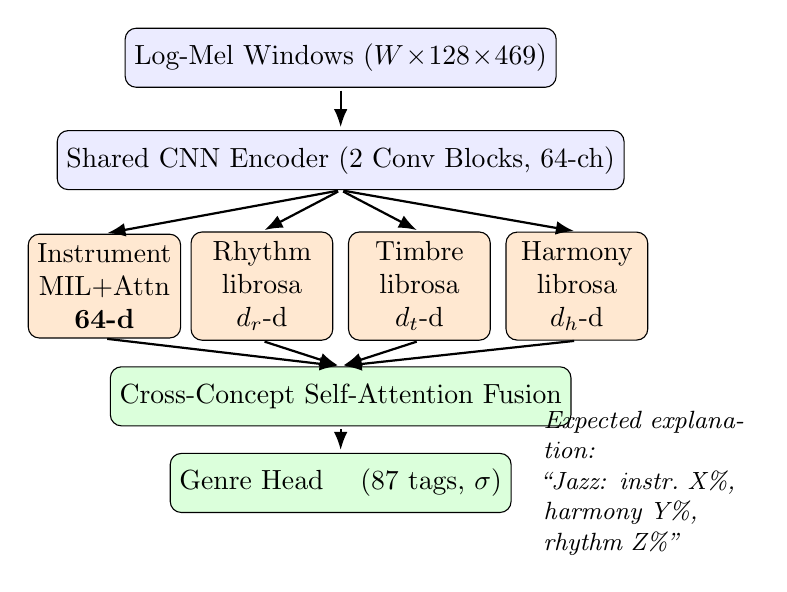
\begin{tikzpicture}[
  box/.style={draw, rounded corners=4pt, fill=blue!8,
              minimum width=4.2cm, minimum height=0.75cm,
              font=\normalsize, align=center},
  cbox/.style={draw, rounded corners=4pt, fill=orange!18,
               minimum width=1.8cm, minimum height=1.1cm,
               font=\normalsize, align=center},
  fbox/.style={draw, rounded corners=4pt, fill=green!14,
               minimum width=4.2cm, minimum height=0.75cm,
               font=\normalsize, align=center},
  arr/.style={-Latex, thick, shorten >=1pt, shorten <=1pt}
]
%% Input and shared encoder — centred at x=0
\node[box] (input) at (0, 0)    {Log-Mel Windows $(W\!\times\!128\!\times\!469)$};
\node[box] (cnn)   at (0,-1.3)  {Shared CNN Encoder (2 Conv Blocks, 64-ch)};
\draw[arr] (input) -- (cnn);

%% Four concept boxes evenly spaced at x = -3, -1, +1, +3
\node[cbox] (inst) at (-3.0,-2.9) {Instrument\\MIL+Attn\\\textbf{64-d}};
\node[cbox] (rhyt) at (-1.0,-2.9) {Rhythm\\librosa\\$d_r$-d};
\node[cbox] (timb) at ( 1.0,-2.9) {Timbre\\librosa\\$d_t$-d};
\node[cbox] (harm) at ( 3.0,-2.9) {Harmony\\librosa\\$d_h$-d};

%% Arrows: CNN south → each concept box north
\draw[arr] (cnn.south) -- (inst.north);
\draw[arr] (cnn.south) -- (rhyt.north);
\draw[arr] (cnn.south) -- (timb.north);
\draw[arr] (cnn.south) -- (harm.north);

%% Fusion layer
\node[fbox] (fuse) at (0,-4.3) {Cross-Concept Self-Attention Fusion};

%% Arrows: each concept box south → fusion north
\draw[arr] (inst.south) -- (fuse.north);
\draw[arr] (rhyt.south) -- (fuse.north);
\draw[arr] (timb.south) -- (fuse.north);
\draw[arr] (harm.south) -- (fuse.north);

%% Genre head
\node[fbox] (head) at (0,-5.4) {Genre Head \quad (87 tags,\ $\sigma$)};
\draw[arr] (fuse) -- (head);

%% Example explanation note (placeholder)
\node[font=\small, right=0.3cm of head, text width=2.6cm, align=left]
  {\textit{Expected explanation:\\``Jazz: instr.\ X\%,\\harmony Y\%,\\rhythm Z\%''}};
\end{tikzpicture}%
}% end resizebox
\caption{Proposed concept-guided architecture. Instrument supervision comes from
MTG-Jamendo instrument tags (no extra labelling). Rhythm, timbre, and harmony are
derived from librosa without GPU training. The attention weight matrix
$\mathbf{W}_{\!\text{cpt}}$ yields per-concept genre contributions directly.}
\label{fig:arch}
\end{figure}

\subsection{Stage~1: Instrument Concept Embedding (MIL)}

The proposed instrument module learns a 64-dimensional song-level embedding under multi-label
supervision from the 40 MTG-Jamendo instrument tags. Each song is treated as an ordered bag of
$W$ spectrogram windows. A shared CNN encodes each window $x_j$ to a 64-d feature $\mathbf{h}_j$.
A scalar attention score $s_j=\mathbf{w}^{\!\top}\mathbf{h}_j$ is computed per window; padded
windows are masked before softmax; the song embedding is the attention-weighted sum:
\begin{equation}
  \mathbf{z} = \sum_{j=1}^{W} \alpha_j\,\mathbf{h}_j,\qquad
  \alpha_j = \frac{\exp(s_j)\cdot m_j}{\sum_{k}\exp(s_k)\cdot m_k},
\end{equation}
where $m_j\in\{0,1\}$ is the validity mask. A final linear head maps $\mathbf{z}$ to 40
instrument logits, optimised with \texttt{BCEWithLogitsLoss}. The weights $\{\alpha_j\}$ will
additionally identify which 15-second segment most influenced each instrument prediction,
constituting a built-in temporal explanation layer. Table~\ref{tab:arch} summarises all layer dimensions for this stage.

\begin{table}[h]
  \caption{Stage~1 MIL model layer dimensions.}
  \label{tab:arch}
  \begin{tabular}{llr}
    \toprule
    Layer & Output shape & Params \\
    \midrule
    Input (per window)           & $1\!\times\!128\!\times\!469$ & --- \\
    Conv2D-32 + ReLU + MaxPool   & $32\!\times\!64\!\times\!234$ & 320 \\
    Conv2D-64 + ReLU + AvgPool   & $64\!\times\!1\!\times\!1$    & 18,496 \\
    Linear projection (64-d)     & $64$                          & 4,160 \\
    Attention score              & scalar                        & 65 \\
    Attention-weighted sum       & $64$                          & --- \\
    Instrument head (40 tags)    & $40$                          & 2,600 \\
    \midrule
    \textbf{Total}               &                               & \textbf{25,641} \\
    \bottomrule
  \end{tabular}
\end{table}

\subsection{Rhythm Concept Extraction}

The rhythm concept will be captured by extracting temporal and percussive features per 15-second window using \texttt{librosa}. This includes the estimated tempo (in BPM), overall beat strength, onset density, and beat-interval statistics (mean and standard deviation of inter-beat intervals). These features are aggregated to a song-level representation by concatenating the per-window mean and standard deviation, providing a robust summary of the track's rhythmic structure.

\subsection{Timbre Concept Extraction}

Timbral characteristics, which describe the color or texture of the sound independently of pitch and loudness, will be extracted via a comprehensive set of spectral features. For each window, we compute the spectral centroid, bandwidth, spectral contrast across seven sub-bands, spectral flatness, RMS energy, and spectral flux. The song-level timbre vector is formed by concatenating the mean and standard deviation of these features across all windows.

\subsection{Harmony Concept Extraction}

To capture the harmonic and tonal content of the music, we extract a 12-dimensional chroma vector and a 6-dimensional Tonn\'{e}tz projection for each 15-second window. The chroma features represent the energy distribution across the twelve pitch classes, while the Tonn\'{e}tz features map harmonic relations onto a topological space. These are aggregated into a song-level harmony vector using the mean and standard deviation.

Before fusion, all rhythm, timbre, and harmony features will be $z$-score normalised using training-split statistics to ensure uniform scaling.

\subsection{Stage~2: Attention Fusion and Genre Head}

The four concept vectors will be projected to a common token dimension via independent linear
layers and concatenated into a sequence of four tokens passed through single-head self-attention:
\begin{equation}
  \mathbf{T} = [\mathbf{p}_{\text{inst}},\,\mathbf{p}_r,\,\mathbf{p}_t,\,\mathbf{p}_h]
               \in\mathbb{R}^{4\times64},
\end{equation}
\begin{equation}
  \hat{\mathbf{T}},\,\mathbf{W}_{\!\text{cpt}} = \operatorname{MHA}(\mathbf{T},\mathbf{T},\mathbf{T}),
\end{equation}
where $\mathbf{W}_{\!\text{cpt}}\in\mathbb{R}^{4\times4}$ is the cross-concept attention weight
matrix. Specifically, the attention mechanism computes query ($\mathbf{Q}$), key ($\mathbf{K}$), and value ($\mathbf{V}$) matrices using learned projections of the token sequence $\mathbf{T}$, followed by scaled dot-product attention:
\begin{equation}
  \operatorname{Attention}(\mathbf{Q},\mathbf{K},\mathbf{V}) = \operatorname{softmax}\left(\frac{\mathbf{Q}\mathbf{K}^{\top}}{\sqrt{d_{\text{tok}}}}\right)\mathbf{V}.
\end{equation}
This formulation explicitly models cross-concept relationships (e.g., how the presence of specific instruments correlates with high rhythmic density or particular harmonic structures). The resulting matrix $\mathbf{W}_{\!\text{cpt}} = \operatorname{softmax}(\mathbf{Q}\mathbf{K}^{\top}/\sqrt{d_{\text{tok}}})$ captures the exact percentage contribution of each concept to the final prediction.

After the attention operation, the mean-pooled sequence representation $\bar{\mathbf{t}}\in\mathbb{R}^{64}$ passes through a two-layer MLP (ReLU, Dropout~0.2, $d_{\text{fused}}=128$), and a final linear layer predicts 87 genre logits with sigmoid activations.

%%─────────────────────────────────────────────
\section{Evaluation Plan and Expected Results}

As this is a proposed architecture, comprehensive empirical evaluation is slated for future work.
We outline our evaluation methodology and anticipated outcomes below.

\subsection{Preliminary Baseline Results}

We have implemented the standard CNN architecture~\cite{hershey2017cnn} trained end-to-end for genre
tagging independently of any concept supervision to serve as our primary baseline. Both the
baseline and our proposed architecture will be evaluated on the held-out \texttt{split-0} test
set, reporting macro ROC-AUC and macro PR-AUC.

\begin{table}[h]
  \caption{CNN baseline test-set results (split-0). Batch 64 exceeded T4 VRAM on every
           attempt and is excluded.}
  \label{tab:baseline}
  \begin{tabular}{lccc}
    \toprule
    Task & Batch & ROC-AUC & PR-AUC \\
    \midrule
    Genre (87 tags)      & \textbf{16} & \textbf{0.7260} & \textbf{0.1592} \\
    Genre (87 tags)      & 32          & 0.6916          & 0.1373          \\
    Instrument (40 tags) & 32          & 0.6417          & 0.1678          \\
    \bottomrule
  \end{tabular}
\end{table}

Batch size 16 outperforms batch 32 by $+$0.034 ROC-AUC and $+$0.022 PR-AUC, suggesting that
more frequent gradient updates are beneficial given the small subset size and highly imbalanced
multi-label target distribution. The batch-16 genre configuration serves as the primary
comparison point for all concept-guided experiments.

\subsection{Expected Accuracy--Interpretability Tradeoff}

The accuracy--interpretability tradeoff is the central tension of concept-bottleneck
approaches~\cite{koh2020concept}: forcing predictions through a human-defined concept layer
imposes an information bottleneck that constrains the representational capacity available to the
final classification head. Consequently, \textbf{we expect the proposed concept-guided model to
achieve lower predictive accuracy (ROC-AUC / PR-AUC) than the unconstrained CNN baseline.}

This anticipated performance drop is an accepted cost of the architecture. By trading some
predictive power for structural constraints, the concept bottleneck ensures that every genre
prediction is auditable. The experimental phase will aim to quantify this gap and demonstrate
that it remains within an acceptable margin for practical application.

\subsection{Planned Ablations}

To understand the contribution of each component, we plan to evaluate the following ablations:
\begin{itemize}[leftmargin=*]
  \item \textbf{Concept additions}: Sequentially adding Rhythm, Timbre, and Harmony features
        to the Instrument-only model. We anticipate each additional concept module will provide
        a consistent, additive improvement in predictive metrics.
  \item \textbf{Fusion mechanism}: Comparing linear concatenation against the proposed
        cross-concept attention fusion. We expect attention fusion to outperform simple
        concatenation by capturing interactions between concept streams (e.g., the relationship
        between harmonic complexity and instrument presence).
\end{itemize}

\subsection{Expected Explainability Capabilities}

The primary advantage of the proposed architecture over the baseline is its capability to produce
two complementary explanation layers inherently, without post-hoc approximation:

\textbf{Layer 1 --- Concept-level contributions.}
The cross-concept attention weight matrix $\mathbf{W}_{\!\text{cpt}}$ will assign each of the
four concept streams a contribution score for every genre decision. For example, we anticipate
that predictions for \textit{Classical} will be dominated by instrument identity and harmony,
while \textit{Electronic} will foreground timbre and rhythm.

\textbf{Layer 2 --- Temporal salience.}
The per-window attention weights $\{\alpha_j\}$ of the MIL encoder will identify which 15-second
segment most influenced each instrument prediction, enabling direct verification against audible
content.

%%─────────────────────────────────────────────
\section{Proposed Practical Applications}

The transparent nature of the proposed CBM architecture enables practical applications that are structurally impossible with traditional black-box classifiers. We highlight two key use cases that will be explored in future work.

\subsection{Auditable Content Tagging}

In commercial streaming platforms, automated tagging errors can have significant financial and legal consequences (e.g., misclassifying explicit content or incorrectly assigning genre metadata that impacts royalty distributions). A standard CNN baseline cannot provide an auditable trail for its decisions. In contrast, our proposed architecture guarantees that every genre prediction is explicitly routed through the four-concept bottleneck. If a track is classified as \textit{Jazz}, a musicologist or content auditor can directly inspect the attention weights (Layer 1) to see that the decision was driven heavily by the \textit{Instrument} stream. Furthermore, the auditor can trace the instrument prediction down to the specific 15-second window (Layer 2) that the model attended to most strongly. This provides a clear, actionable audit trail.

\subsection{Human-in-the-Loop Interventions}

Because the concepts in our bottleneck correspond to human-understandable musical properties, the model supports direct, targeted interventions~\cite{koh2020concept}. If a human auditor reviews the output and notices that the model mistakenly identified \textit{Electronic} instead of \textit{Acoustic} instruments due to recording distortion, they can manually correct the instrument logits. The corrected instrument vector can then be passed forward through the frozen Stage 2 fusion module to yield an updated, corrected genre prediction without requiring any retraining of the neural network. This capability is uniquely valuable for maintaining high-quality metadata catalogues where human reviewers can safely override intermediate errors.

%%─────────────────────────────────────────────
\section{Conclusion}

We have proposed a four-concept bottleneck architecture for explainable music genre
classification that routes predictions through musically meaningful intermediate representations:
instrument presence, rhythm, timbre, and harmony. While we expect this constrained design to
yield slightly lower predictive accuracy compared to a standard end-to-end CNN baseline, it
promises to provide transparent, instrument-grounded genre explanations that black-box models
cannot produce. Future work will focus on implementing the architecture, executing the outlined
training protocol on MTG-Jamendo \texttt{split-0}, quantifying the accuracy--interpretability
tradeoff, and conducting a formal evaluation of the generated explanations.

\bibliographystyle{ACM-Reference-Format}
\bibliography{dnn}

\end{document}
